\chapter{Introduction}
\emph{The chapter starts with a background describing who Trafikverket are and why Road Weather Information Systems are used and why the technology behind them needs improvement. This is followed up with explaining machine learning basics are explained and how machine learning can be used in this project. Lastly, an objective for the project is defined followed by its delimitations. }
%Lastly, a thesis structure is presented to simplify navigation through different parts of the project.}

\section{Background} \label{sec:background}
	Living in cold areas of the world typically means an increased amount of work for invididual people, municipalities and companies in trying to maintain a non-winter-like infrastructure. This of course, also involves winter road maintenance. Salting and plowing roads is an investment in not only saving lives, but also in lowering socio-economic costs; Arvidsson \cite{ARTICLE:1} presents two scenarios which explains this claim: The two scenarios take place on a road with 2 cm snow and a daily traffic flow of 2000 vehicles, one with a salted and ploughed road taking four hours to drive, and the other scenario on the same road without winter maintenance taking five hours to drive. Arvidson argues that the total socio-economic costs are 3.5\% higher in the non-maintained road, mainly due to increased travel time and thus, higher accident costs. 


	\subsection{Road Weather Information Systems}
	While the socio-economic savings in performing winter road maintenance may be enough to justify the need for it, winter road maintenance can still present a notable economic cost for the organization(s) involved. Trafikverket, the agency in charge of state road maintenance in Sweden, reported that winter road maintenance were roughly 18\% of the total road maintenance costs in 2013 \cite{REPORT:1}. Local contracters are hired to carry out the plowing and salting of state roads, with requirements on both ends regarding when to plow, which roads to prioritize etc. \cite{WEBSITE:2}. Trafikverket help contracters monitor road conditions with their so-called Road Weather Information Systems (RWIS) \cite{WEBSITE:2}. Trafikverket have around 800 RWIS distributed across state roads in Sweden which are used by contracters to carry out winter road maintenance work \cite{WEBSITE:2}. 

\begin{figure}[H]
	\centering
	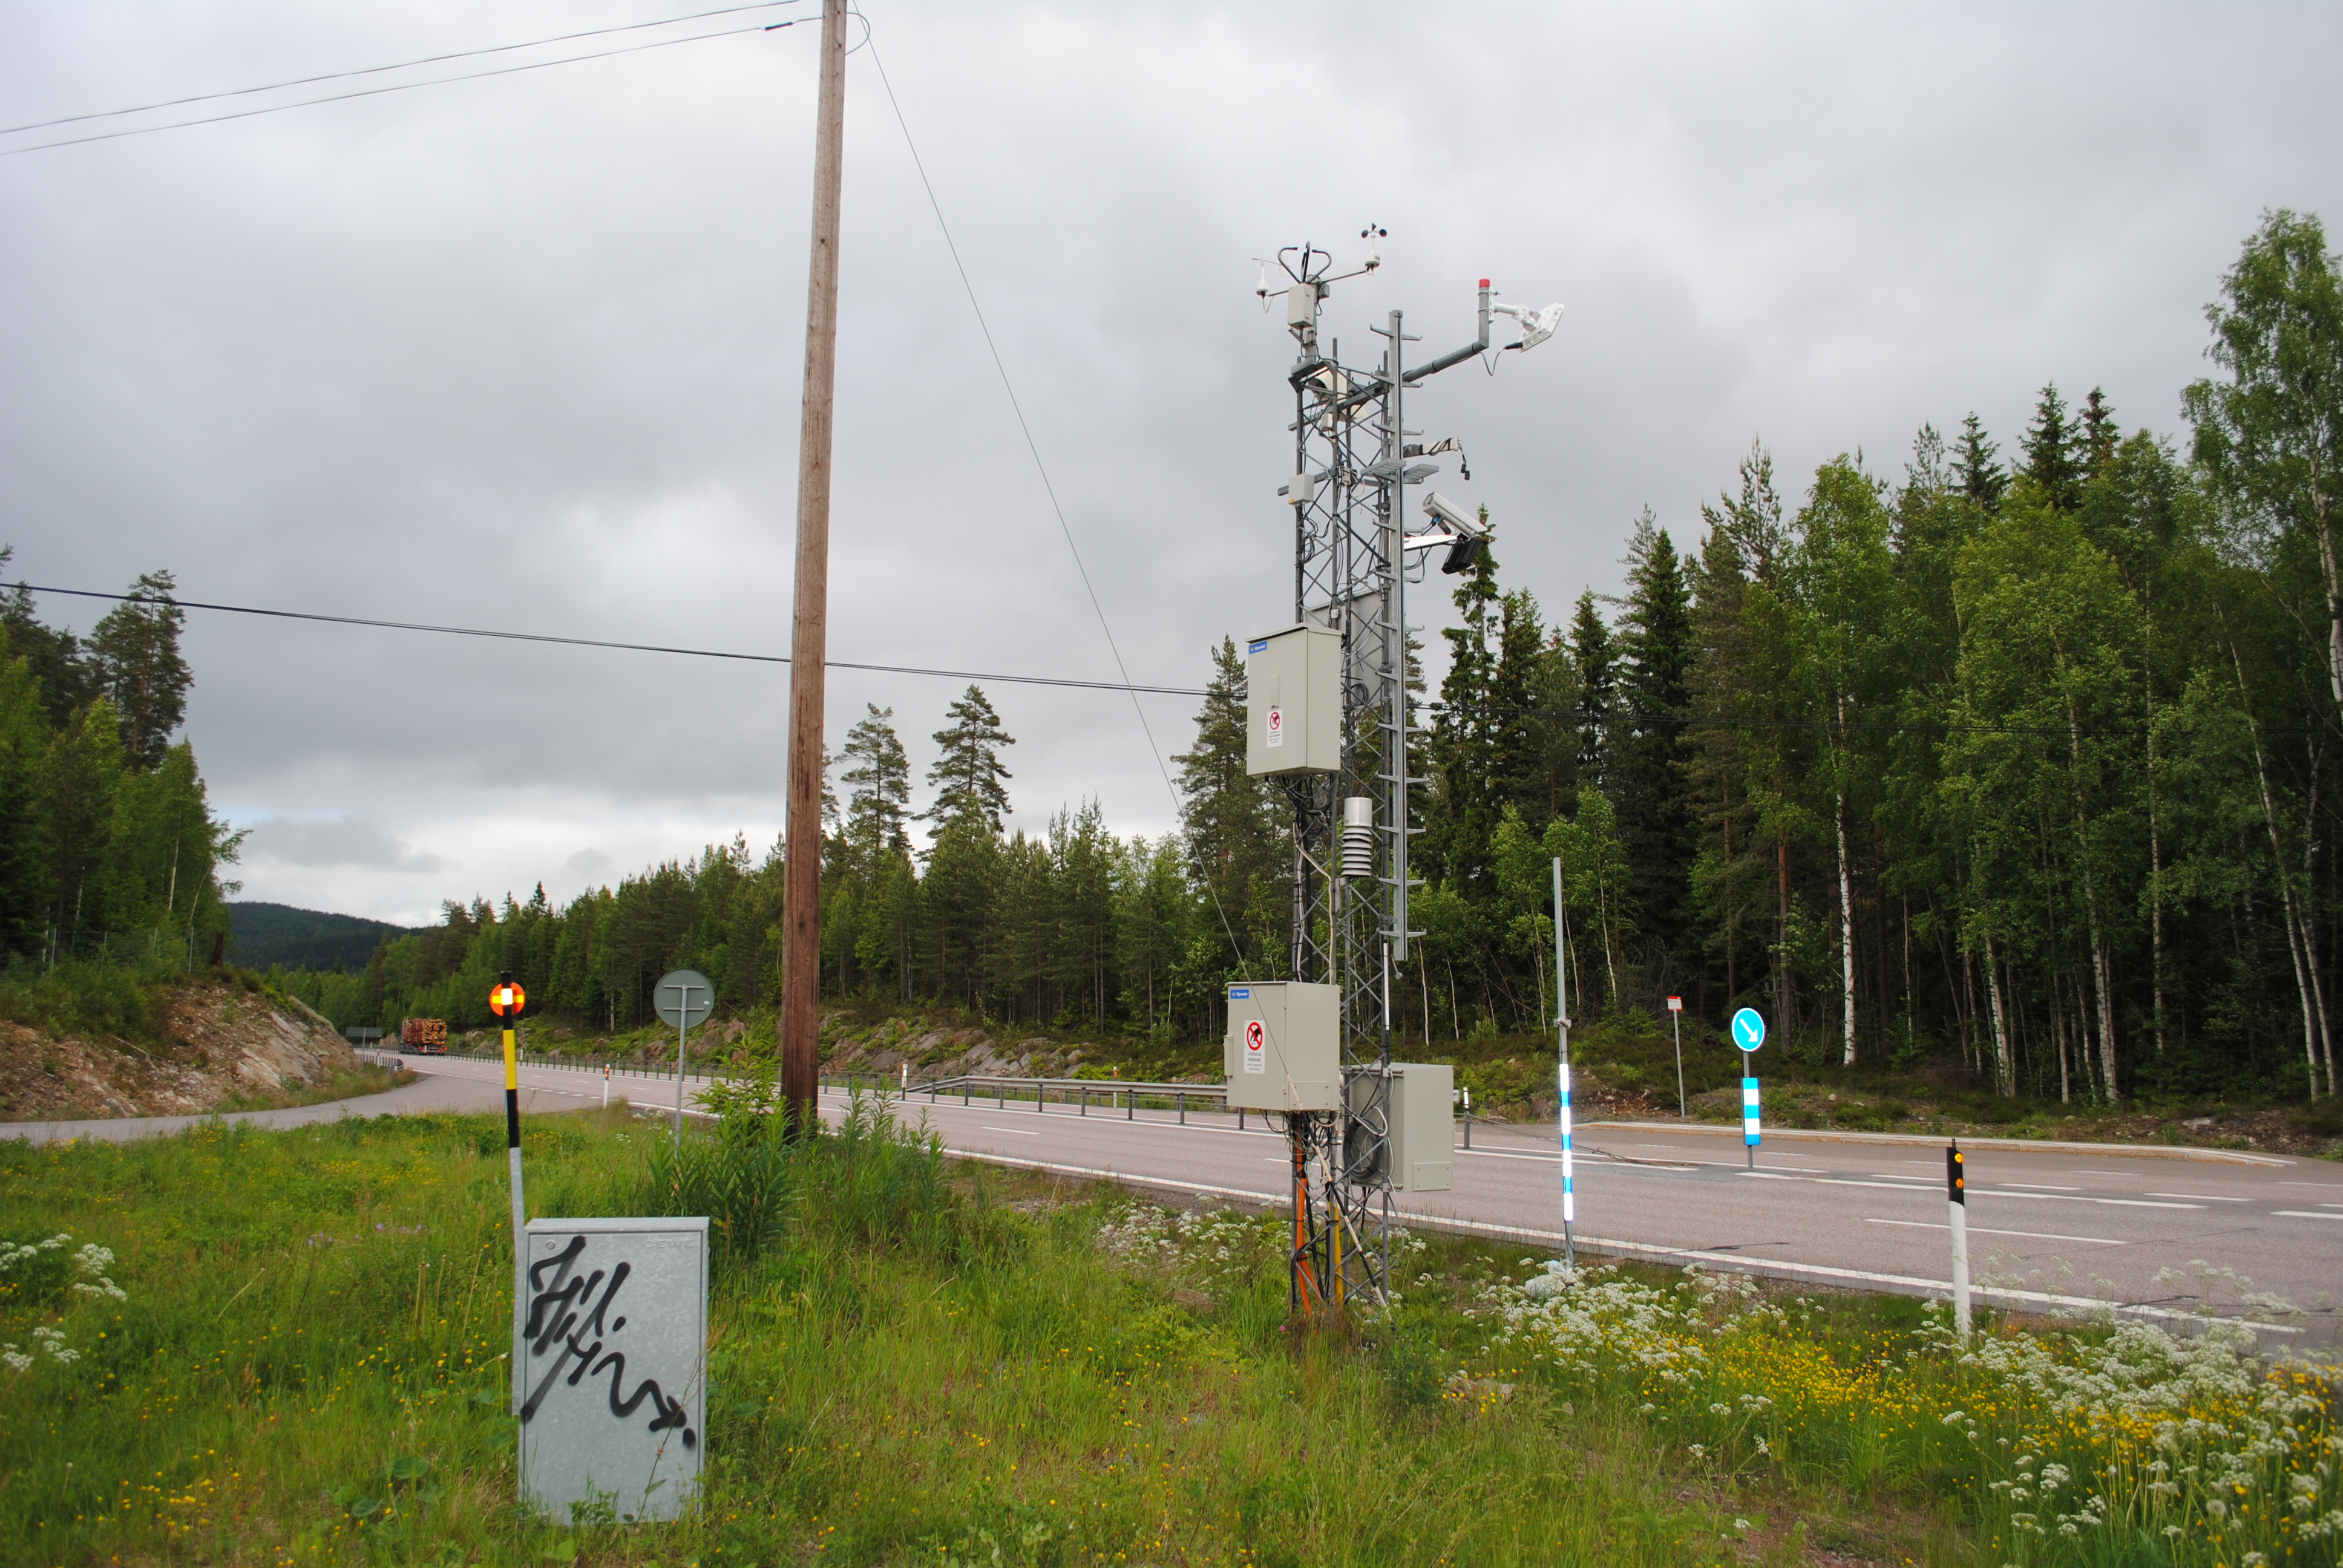
\includegraphics[width=0.8\textwidth]{media/Rwis_station_Myggsjon_01.JPG}
	\caption{RWIS station at sensor site Myggsjön \cite{IMAGE:1}.}
	\label{img:rwis}
\end{figure}

\begin{table}[H]
	\caption{Measurements that are studied in this project from RWIS with corresponding instrument- or sensor names\cite{MAIL:1, REPORT:3}. }
 	\resizebox{\textwidth}{!}{%
		\begin{tabular}[3]{l | l | l | l}
    			Instrument/sensor name & Feature & Value & Measured at how many RWIS  \\
    			\hline
			Optic Eye & precipitation type & discrete & all \\
			Optic Eye & precipitation amount & continous & all \\
			Track Ice Road Sensor & road surface temperature & continous & all \\
			DST111 & road surface temperature & continous & $\sim 7$ \\
			DSC111 & road surface condition & discrete &  $\sim 26$ \\
			DSC111 & road friction & continous & $\sim 26$ \\
			MS4 & timestamp  & date (mmddhhmm) & all 
			\label{table:rwis}
		\end{tabular}
		}
\end{table}

	Table \ref{table:rwis} shows some of the sensors that the operational RWIS are equipped with. In addition to the sensors listed in table \ref{table:rwis}, many of the stations are also equipped with a camera \cite{REPORT:2}. The operational RWIS also measure air humidity, air temperature, max-wind, wind-average and more. The sensors are connected to a nearby computer called MS4. Trafikverket aim to replace MS4 with a new generation of computers by 2021 \cite{REPORT:4}. MS4 has limited capacity to handle current and future contracter needs, and electric components are becoming hard for Trafikverket to replace \cite{REPORT:4}. 

	Over personal communication with Johan Casselgren at Luleå University of Technology, Johan mentions that it is interesting to investigate if certain sensors, especially the Track Ice Road Sensor (TIRS), can be replaced along with the new generation of computers. TIRS is required to be dug into the road, which may require roads to be closed off temporarily during installation. Furthermore, if the sensor is removed, a hole is left in the road which can cause problems. In that way, the DST111 may prove more useful since it measures road temperature remotely using infrared laser \cite{WEBSITE:19}. %but TIRS data still needed? why?
	%efter år 2022 bör inga givare finnas i vägbanan \

	The author, Johan Casselgren and Niklas Karvonen, who is also from Luleå University of Technology, hypothesized over personal communication that machine learning models can probably be used to model the behavior of TIRS. The author and Johan Casselgren also sees potential in using machine learning models as a backup system when sensors malfunction. It is therefore interesting to see if the other sensors from table \ref{table:rwis} can be modelled as well. 

	 %Neither the additional features, nor the road photos taken by the camera are considered in this project since the author hypothesize that the measurements made by the sensors in \ref{table:rwis} are enough to build machine learning models. Adding additional features may also lead to increased amount of errors and higher complexity in introducing the curse of dimensionality (see \ref{sec:machinelearning}). 

%lägg till ref till table som visar att dom failar ganska ofta

	\subsection{Machine learning} \label{sec:machinelearning}
	Machine learning as formally defined by Mitchell \cite{BOOK:2}: 
"A computer program is said to learn from experience $E$ with respect to some class of tasks $T$ and performance measure $P$ if its performance at tasks in $T$, as measured by $P$, improves with experience $E$". This means that machine learning algorithms are used to solve a set of problems, measure its performance in doing so, and ultimately improve in some way from previous experience. For example, imagine a program designed to determine if a human face is in a photo or not. Since photos are taken at different distances, angles and faces have different characteristics such as eye color, skin color, distance between eyes and nose shape, implementing this "manually" may prove cumbersome. Instead of programming an algorithm to recognize faces, it can be programmed  \emph{to learn to recognize faces}. If the algorithm is allowed to analyze a dataset with thousands of photos of human faces, it could learn to distinguish a human face by recognizing parts of the face such as eyes, nose, mouth and where those parts are most likely placed to oneanother.

	In essence, machine learning algorithms improve/learn in some way from analyzing a dataset. How they learn can be used to broadly categorize machine learning algorithms as either having supervised or unsupervised learning \cite{BOOK:1}. Supervised learning algorithms process a labeled dataset while unsupervised learning attempts to make sense of unlabeled data. The data provided by Trafikverket to perform this project is labeled data in the form of column headers in Microsoft Excel workbooks (see provided data in \ref{sec:provided_data}). 

	Dimensionality in machine learning refers to how many features are used as input to train a machine learning algorithm. A tempting brute-force approach to a machine learning problem may be to include every possible feature available to build a model, not only those brought up in table \ref{table:rwis}, but also road photos, wind-speed etc. This however, may introduce the curse of dimensionality, which basically means that higher dimensional data introduces complexity and possibly an increased amount of errors in the model \cite{BOOK:6}. During a personal meeting, Johan Casselgren also recommended to focus on using the features listed in table \ref{table:rwis}. However, according to Jonas Hallenberg who works at Trafikverket, there are difficulties in trying to model the DSC111 sensor. The problem is that Trafikverket use salt on every road where the DSC111 sensor is, save one, and salt affects the road surface status. So for example, when the surface temperature and dew point temperature suggests that road surface condition is icy, which could be measured by DSC111, it may be wet in reality. Johan casselgren suggests that data from the DSC111 sensor can still be used as input when modelling the other sensors. Data from TIRS road temperature is not to be used as input when modelling remaining sensors since Trafikverket may remove this sensor in the future. 
	
	The forementioned definition of machine learning by \cite{BOOK:2} mentions a performance measure $P$. A performance measure can be used to evaluate a supervised learning algorithm's abilitiy to model a given feature A specific feature that is to be modelled is referred to as target feature, and the features a supervised learning algorithm uses to do so is referred to as input features. In a basic sense, a supervised learning algorithm studies the values of the target feature and attempts to build a model that best fits its behavior based on data from input features. But the algorithm is not necessarily perfect by having a high performance score on its training dataset. If a model is built in such a way that it fits its provided training data perfectly, which may have outliers, errors etc., it may have difficulties in predicting unseen data. This condition is known as overfitting, the opposite: underfitting, both of which are covered in detail in \ref{sec:generalization}. So it is not enough for a supervised learning algorithm to have a high performance, it should also generalize well on unseen data. 

\section{Objective} \label{sec:objective}
	The objective of this thesis is to find optimized supervised learning algorithms, in terms of performance and generalization, which model the behavior of the following sensors: Optic Eye, TIRS and DST111. Each sensor is modelled using measurements made by the other sensors, except for TIRS. Any algorithm may train on the following input features as well: timestamp, road friction and road surface condition. Timestamp is provided by the RWIS computer MS4. Road friction and road surface condition are measured by a sensor called DSC111.
	
	The objective is broken down to four subtasks that are to be solved:
	\begin{enumerate}
		\item Find the algorithm among a set of supervised learning algorithms, that can be used to classify \textbf{precipitation type}, with the best performance- and generalization score. The algorithm may use the following input features: 
			\begin{itemize}
				\item timestamp
				\item DST111 road surface temperature
				\item road friction
				\item road surface condition
			\end{itemize}
		\item Find the algorithm among a set of supervised learning algorithms, that can be used to predict \textbf{precipitation amount}, with the best performance- and generalization score. The algorithm may use the following input features: 
			\begin{itemize}
				\item timestamp
				\item DST111 road surface temperature
				\item road friction
				\item road surface condition
			\end{itemize}
		\item Find the algorithm among a set of supervised learning algorithms, that can be used to predict \textbf{TIRS road surface temperature}, with the best performance- and generalization score. The algorithm may use the following input features: 
			\begin{itemize}
				\item timestamp
				\item precipitation type
				\item precipitation amount
				\item DST111 road surface temperature
				\item road friction
				\item road surface condition
			\end{itemize}
		\item Find the algorithm among a set of supervised learning algorithms, that can be used to predict \textbf{DST111 road surface temperature}, with the best performance- and generalization score. The algorithm may use the following input features: 
			\begin{itemize}
				\item timestamp
				\item precipitation type
				\item precipitation amount
				\item road friction
				\item road surface condition
			\end{itemize}
	\end{enumerate}

\section{Delimitations} \label{sec:delimitations}
	There are many supervised learning algorithms, all of which are not evaluated in detail in this project. An algorithm is qualified for evaluation in this project if the following is true:
	\begin{enumerate}
		\item The algorithm is a supervised learning algorithm that solves regression and/or multiclass classification problems (see \ref{sec:classification} and \ref{sec:regression})
		\item The algorithm is available in Scikit-learn \cite{WEBSITE:15}
		\item The algorithm belongs to one of the following algorithm families (see \ref{sec:supervised_algorithms}):
			\begin{itemize}
				\item Decision tree based learning %cart
				\item Instance based learning %knn
				%\item Kernel methods based learning %svm
				\item Bayesian learning %GaussianNB
				\item Regression based learning %linear regression, logistic regression, lasso?
				\item Artificial Neural Networks %backpropagation
				\item Ensemble learning %random forest
			\end{itemize}
	\end{enumerate}

	The performance of supervised algorithms can generally be improved by optimizing its hyperparameters (see \ref{sec:hyperparameters}). However, there can be many ways that a single algorithm can be configured. This project deals with comparing performances of several algorithms and to explore all combinations of hyperparameter settings is too time-consuming. When it comes to optimizing hyperparameters, it was decided to focus on the choice of $k$ in kNN, the number of hidden nodes in MLP and magnitude of regularization $\lambda$ in Lasso (see \ref{sec:supervised_algorithms} and \ref{sec:regularization}).
 
	Some of the sensors, such as the DSC111 (see figure \ref{img:histogram_surfstatus}), are malfunctioning frequently. To avoid any complex relationships between functioning and malfunctioning sensors, it was decided to model non-error behavior by using non-error input features only. 

	In addition to the timestamp feature, an extra feature was present in the provided dataset which displayed what year each observation was taken. The author assumes that global warming does not present a significant change in weather conditions, road surface temperature etc. Furthermore, since the measurements are from 2015-2016, it is assumed by the author that any model built using year as an input feature could potentially do well when dealing with new observations whose year is 2015 or 2016, but that it generalizes poorly when dealing with observations from 2018 or other years. By these assumptions, it was decided to not consider year as an input feature. 

	Support vector machine (SVM) algorithms could have been evaluated in this project, but was ruled out since they appear to have high computational running-time. It was revealed by the author, through a cross-validation classification spot-checking test (see \ref{sec:exp_setups}) on the iris dataset in Scikit-learn, that SVM algorithms have significantly longer running-time than the other algorithms from table \ref{table:evaluated_algorithms}.

\section{Provided data} \label{sec:provided_data}
	A dataset containing 171425 measurements (observations) was provided by Jonas Hallenberg at Trafikverket to carry out this project. The observations are from 2015-2016 from six RWIS along state road E6 in Sweden. The stations measure the features seen in table \ref{table:rwis} making one measurement every ~30 minutes. Six Microsoft Excel workbooks represent data from each of the six stations, in which the column headers are the features seen in table \ref{table:rwis}. The year each observation was taken is also represented in a column in the workbooks.

	A readme.txt file was also provided. It explains in words how to interpret the observations. As can be seen in table \ref{table:rwis}, precipitation type and road surface condition have discrete values that are explained in the readme file. Table \ref{table:discretevalues} shows what each value corresponds to.
		
\begin{table}[H]
	\centering
	\caption{Values that Optic Eye precipitation type and DSC111 road surface condition can assume and what they mean.}
		\begin{tabular}[3]{c | c | c}
    			Value & Precipitation type & Road surface condition \\
    			\hline
			-9 & missing sensor/error & - \\
			0 & - & error\\
			1 & no precipitation & dry \\
			2 & rain with $>= 0 \celsius$ air temperature & moist \\
			3 & rain with $< 0 \celsius$ air temperature & wet \\
			4 & snow & - \\
			5 & - & frost \\
			6 & rain and snow mixed  & snow \\
			7 & - & ice \\
			9 & unknown type  & slush 
			\label{table:discretevalues}
		\end{tabular}
\end{table}

%\section{Thesis structure}
% explain what the thesis looks like
